\documentclass[12pt,a4wide]{report}

\usepackage{amsthm,amssymb,mathrsfs,setspace,pstcol}%amsmath, latexsym,footmisc

\usepackage{play}
\usepackage{epsfig}
%\usepackage[grey,times]{quotchap}
\usepackage[nottoc]{tocbibind}
\renewcommand{\chaptermark}[1]{\markboth{#1}{}}
\renewcommand{\sectionmark}[1]{\markright{\thesection\ #1}}
%

\input xy
\xyoption{all}


\theoremstyle{plain}
\newtheorem{theorem}{Theorem}[section]
\newtheorem{lemma}[theorem]{Lemma}
\newtheorem{corollary}[theorem]{Corollary}
\newtheorem{proposition}[theorem]{Proposition}

\theoremstyle{definition}
\newtheorem{definition}[theorem]{Definition}
\newtheorem{example}[theorem]{Example}
\newtheorem{notation}[theorem]{Notation}

\theoremstyle{remark}
\newtheorem{remark}[theorem]{Remark}

\renewcommand{\baselinestretch}{1.5}
\begin{document}

%\pagenumbering{arabic} \setcounter{page}{1}

% --------------- Title page -----------------------
\begin{titlepage}
\enlargethispage{5cm}

\begin{center}

\vspace*{-1cm}

\textbf{\Large AI-Driven Driver Drowsiness Detection System: A Deep Dive into Model Enhancement and Application}\\[10pt]

\vspace*{2 cm}


            
A Project Report Submitted \\
in Partial Fulfilment of the Requirements  \\
for the Degree of  \\
     \vspace{4.5mm}
{\Large \bf BACHELOR OF TECHNOLOGY } \\
in \\
{\large \bf COMPUTER SCIENCE AND ENGINEERING } \\

 \vspace{9mm}
{\em  by} \\ \vspace{2.5mm}
             {\large \bf MOHD AMMAR - 2021BCS0082 } \\ 
             {\large \bf ROHAN GUDIMETLA - 2021BCS0015 } \\ 
             {\large \bf P PUJA - 2021BCS0198 } \\ 
             {\large \bf BOYINA NITHIN - 2021BCS0088 } \\

\vfill
%\includegraphics[width=12cm, height=12cm]{iiserlogo}

\begin{figure}[h]
% \includegraphics[width=15mm,height=10mm]{time_arma_gs.jpg}
  \begin{center}
  
\includegraphics[width=6cm, height=3cm]{logo2.jpg}
  \end{center}
\end{figure}
\vspace*{0.2cm}
{\em\large to }\\%[8pt]
{\bf \mbox{DEPARTMENT OF COMPUTER SCIENCE AND ENGINEERING}} \\%[4pt]
{\bf \mbox{INDIAN INSTITUTE OF INFORMATION TECHNOLOGY}}\\%[4pt]
{\bf KOTTAYAM-686635, INDIA}\\%[8pt]
{\it November 2024}

\end{center}

\end{titlepage}

\clearpage
% --------------- Declaration  page -----------------------
\pagenumbering{roman} \setcounter{page}{2}
\begin{center}
{\large{\bf{DECLARATION}}}
\end{center}
%\thispagestyle{empty}


\noindent We, \textbf{MOHD AMMAR} (\textbf{Roll No: 2021BCS0082}), \textbf{ROHAN GUDIMETLA} (\textbf{Roll No: 2021BCS0015}), \textbf{P PUJA} (\textbf{Roll No: 2021BCS0198}), \textbf{BOYINA NITHIN} (\textbf{Roll No: 2021BCS0088})  hereby declare that this report entitled
\textbf{``An Academia Recommendation System using Community Detection based on GEAM in Multiplex Networks''} submitted to Indian
Institute of Information Technology Kottayam towards partial
requirement of {\bf Bachelor of Technology} in \textbf{Computer Science Engineering}
is an original work carried out by us under the supervision of
\textbf{Dr. Lidya Lily Thampi} and has not formed the basis for the award
of any degree or diploma, in this or any other institution or
university. We have sincerely tried to uphold the academic ethics
and honesty. Whenever an external information or statement or
result is used then, that have been duly acknowledged and cited.

\vspace{4cm}

\noindent Kottayam-686635 
\hfill 
\textbf{MOHD AMMAR - Roll No: 2021BCS0082}
\noindent November  2024
\hfill
\textbf{ROHAN GUDIMETLA - Roll No: 2021BCS0015}
\rightline{\textbf{P PUJA - Roll No: 2021BCS0198}}
\rightline{ \textbf{BOYINA NITHIN - Roll No: 2021BCS0088}}
\clearpage


% --------------- Certificate page -----------------------
\pagenumbering{roman} \setcounter{page}{3}
\begin{center}
{\large{\bf{CERTIFICATE}}}
\end{center}
%\thispagestyle{empty}


\noindent This is to certify that the work contained in this
project report entitled \textbf{``An Academia Recommendation System using
Community Detection based on GEAM in
Multiplex Networks''}
submitted by \textbf{MOHD AMMAR} (\textbf{Roll No: 2021BCS0082}), \textbf{ROHAN GUDIMETLA} (\textbf{Roll No: 2021BCS0015}), \textbf{P PUJA} (\textbf{Roll No: 2021BCS0198}), \textbf{BOYINA NITHIN} (\textbf{Roll No: 2021BCS0088}) to the Indian Institute of Information Technology Kottayam
towards partial requirement of {\bf Bachelor of
Technology} in
\textbf{Indian Institute
of Information Technology, Kottayam} has been carried out by them under my supervision and that it has not been submitted elsewhere for the
award of any degree.


\vspace{4cm}

\noindent Kottayam-686635  \hfill (Dr. Lidya Lily Thampi)

\noindent November  2024 \hfill Project Supervisor

\clearpage




% --------------- Abstract page -----------------------
\begin{center}
{\Large{\bf{ABSTRACT}}}
\end{center}

The paper introduces an AI-Driven driver drowsiness detection system that aims to utilize two base models --- (i) one that utilizes a shallow convolutional neural network (CNN) with novel transfer learning-based features which combines the strengths of the Visual Geometry Group (VGG-16) and Light Gradient-Boosting Machine (LGBM) methods (ii) other that uses a multi-loss convolutional neural network. These models are ensembled through stacked generalization to enhance the drowsiness detection.

The first base model predicts driver drowsiness using eye movement behaviour, and opening and closing of the eye lids. First, a 68-point face landmark identification approach is
used to identify faces and extract the eye areas. Then, these are passed through a lightweight CNN model, powered by VGG which  generates salient transfer features using LGBM. A K-Neighbour classifier is used to detect the drowsiness using the features extracted.

The second base model utilizes a multi-loss convolutional neural network pre-trained on 300W-LP, a large synthetically expanded dataset, to predict the Euler angles of head --- pitch, roll, and yaw directly from the images,  through joint binned pose classification and regression. Then, excessive deviation of driver's head posture is detected using an empirical relation among the Euler angles, to detect driver drowsiness.

Ensemble techniques like stacked generalization is utilized to improve overall predictive performance by leveraging the strengths of each model variant.

Overall, the system utilizes a lightweight CNN powered by VGG and LGBM methods to detect drowsiness from facial features, and aims to ensemble it with a multi-loss CNN to detect drowsiness from head posture, aiming to provide a robust system to detect drowsiness in driver, so as to alert the drivers to lower the number of accidents caused by weariness.

\clearpage


\pagenumbering{roman}
\setcounter{page}{5}


\clearpage

\tableofcontents
\clearpage

\section*{List of Figures}

\begin{itemize}
    \item[3.1] Model Architecture \dotfill 15
    \item[3.2]
    \dotfill 37
\end{itemize}
\clearpage

\clearpage

\pagenumbering{arabic}
\setcounter{page}{1}

% --------------- Abstract page -----------------------
% \input abstract.tex

% =========== Main chapters starts here. Type in separate files and include the filename here. ==
% ============================

\chapter{Introduction}

\section{Background}

In today's fast-paced world, where everyone is constantly juggling  around work, social commitments, and personal responsibilities, getting enough sleep has become a luxury. This has taken a significant toll on several people's mental health, so much that the weariness can have extreme consequences when they get behind the wheel. Driving when drowsy significantly impairs reaction times, reduces alertness, and increases the risk of accidents.

As per approximations furnished by the National Highway Traffic Safety Administration (NHTSA), driving while fatigued caused \$12.5 billion in economic loss, 71,000 injuries, and 1,550 fatalities. Statistics (NHTSA) [1] show that in 2017, accidents involving drowsy drivers resulted in 50,000 injuries and 795 fatalities. This calls for the need of a system in the vehicle, which can scan and alert the driver when signs of fatigue are recognized.

One of the most accurate ways of detecting fatigue in driver is through physiological signals like heart rate, Electroencephalography (EEG), Electrocardiography (ECG or EKG), Respiration Rate, Body Temperature, etc. However, these methods are not really feasible, since they require expensive equipment, and a continuous direct contact with driver's body. Hence, we require a system that can detect drowsiness in driver through behavioral signals like eyes movement, opening and closing of mouth, head position, etc. 

To address these challenges, We propose a lightweight novel transfer learning-based features generation which combines the strengths of the Visual Geometry Group (VGG-16) and Light Gradient-Boosting Machine (LGBM) methods. Experimental evaluations reveal that the k-neighbors classifier on the extracted features of eye lids outperformed the state-of-the-art approach with a high-performance accuracy of 99\%. The computational complexity analysis shows that the proposed approach detects driver drowsiness in 0.00829 seconds [2].

However, predicting drowsiness just through facial features and triggering an alarm would seem some what a too bit far-fetched, and might result in certain False Positives. Hence, we aim to top it off by ensembling another multi-loss CNN to it, which estimates the Euler angles (pitch, roll, and yaw) of the driver's head, and use an empirical relation to determine excessive deflection of head. Through this interdisciplinary approach the system aims to combine the accuracies of individual models, and predict driver's fatigue with a greater accuracy.


\vspace{10in}
\section{Goal}
The main objectives of the work are:
\begin{itemize}

    \item Develop an integrated system comprising of an LGBM and a VGG based CNN model to detect driver drowsiness from facial features, coupled using ensemble techniques with another multi-loss CNN model which predicts extreme deflection in driver's head for enhanced accuracy.

    \item Make the model as lightweight as possible, to make it robust and efficient so that it can be incorporated in day-to-day lives.

    \item Incorporate a mechanism for the system to continuously learn and adapt to new data

    \item Fine tune the ensembled model for greater accuracies.

\end{itemize}

\section{Motivation}
In today's fast-paced world, with everyone is constantly juggling  around work, social commitments, and personal responsibilities it becomes absolutely important to have a system to detect and alert a driver when he is drowsy, to prevent accidents. Physiological signals are not really feasible, since they require expensive equipment, and a continuous direct contact with driver's body. By leveraging advanced machine learning techniques like a novel transfer
learning-based features generation with VGG and LGBM in a lightweight convolutional neural network, coupled with ensemble methods, we aim to enhance prediction accuracy and provide accurate signals for drowsiness detection. Making the model lightweight, robust and efficient to consume less energy makes it more usable in real-world scenarios.

\section{Problem Statement}

Develop and evaluate an advanced driver drowsiness detection system that integrates multiple detection techniques to enhance its accuracy and robustness. The system should combine various measures, such as physiological, behavioural, and vehicle-based indicators, to identify drowsiness at different stages. This research will explore and compare different technologies and algorithms, including those based on eye activity, to assess their effectiveness in real-world conditions. The aim is to improve early drowsiness detection, minimize false positives and negatives, and provide insights into integrating these systems into broader driver assistance technologies to enhance overall road safety.



\documentclass[a4paper,12pt]{report}
\usepackage{setspace} % For controlling line spacing
\usepackage{amsmath, amsthm, amssymb} % For mathematical symbols and environments
\usepackage{graphicx} % For including figures
\usepackage{hyperref} % For clickable references
\usepackage{cite} % For citation management

% Theorem-like environments
\newtheorem{theorem}{Theorem}[section]
\newtheorem{definition}{Definition}[section]
\newtheorem{corollary}{Corollary}[theorem]
\newtheorem{remark}{Remark}[section]

\begin{document}
\onehalfspacing

\chapter{Literature Survey}

The paper[3] presents a new method for fatigued driving using a deep learning model that combines the lightweight nature of YOLOv5s with 3D facial key feature extraction. This study shows that the improved YOLOv5 architecture, equipped with ShuffleNetV2\_BD and maxpool cross-scale feature aggregation (M-CFAM), improves the detection accuracy while reducing the computational cost. Vital signs such as Early Response Rate (EAR) and Marginal Response Rate (MAR) are evaluated for important fatigue indicators such as eyes closed and yawning.
The paper notes that PERCLOS (percentage of eyes closed) is useful in detecting fatigue in the short term. However, the long-term monitoring or intervention effects of different factors on the working model are also discussed.
In addition, this model primarily focuses on immediate detection and does not consider the influence of different lighting conditions or environmental factors that may affect the accuracy in real-world use. The focus is on additional measures and other factors that may affect the reliability of driving fatigue intensification.

The paper[4] proposes a hybrid model combining MTCNN for spatial feature extraction and LSTM and TSC-LSTM for temporal sequence analysis (drowsiness detection), enhancing detection accuracy with less noise. The cost computation is compared with original VGG11 architecture to find the fastest and most accurate CNN.

A systematic literature review was conducted to identify studies on eye-activity-based driver drowsiness detection (DDD) systems [5]. Relevant studies were selected from four databases, focusing on drowsiness, eye activity, and performance measures. Key data on ocular parameters, technologies, and performance metrics were extracted and analyzed, with a classification of eye activity measures. Future directions for DDD systems were also discussed.

The study [2] proposed a VGLG approach that combines VGG-16 for feature extraction and LGBM for transfer feature generation. Four machine learning models and two deep neural networks were validated using k-fold cross-validation and hyperparameter tuning. The approach utilized a standard dataset comprising 4,103 eye images of drivers, meticulously labeled as either open or closed eye movements.

The paper [6] suggested a combination of machine learning and deep learning models using HOG features, PCA, and a custom 30-layer CNN architecture. YawDD Video Dataset , with videos of drivers showing normal, talking, and yawning behaviors.

The paper [7] proposed a shallow CNN architecture using limited training data for drowsiness detection based on visual cues like eyelid closure.

Head Pose Estimation Through Euler Angles and Deep LearningRuiz et al. [8] introduce a convolutional neural network (CNN) model that predicts head pose angles—specifically pitch, roll, and yaw—directly from image intensities. This approach bypasses traditional keypoint-based methods, which rely on aligning 2D-3D face models and can be error-prone when landmarks are obscured or inaccurately detected. In Ruiz’s study, the CNN model’s multi-loss function simultaneously classifies and regresses each head pose angle, a method shown to significantly improve accuracy. Using a large, synthetically expanded dataset for training, the model achieves state-of-the-art results on benchmarks such as the AFLW2000 and BIWI datasets.
However, certain limitations are acknowledged, such as a reduction in performance under extreme head poses and on low-resolution images, which points to an ongoing need for robustness improvements, especially for applications like surveillance and driver monitoring.
GRU-Based Temporal Prediction Model for Stock IndicesThe study by [8] proposes StockNet, a GRU-based (Gated Recurrent Unit) model designed to predict stock indices by integrating injection and investigation modules that reduce overfitting through data augmentation. 
StockNet utilizes temporal dependencies within financial time series data, showing that GRU architectures can effectively capture sequential relationships. Despite achieving strong predictive accuracy, StockNet’s reliance on specific data distributions and the need for further generalization to diverse market conditions remain areas for development. The study illustrates the GRU model's capacity to handle complex, time-sensitive financial forecasting tasks, while also suggesting that continuous model adaptation is essential for dynamic financial environments.

The study in [9] described an empirical relation between different Euler angles --- pitch, roll and yaw and extreme deflection of driver's head. As per the study, when the yaw angle is greater than 20°, the pitch angle is greater than 21°, and the roll angle is greater than 20.5°, the driver’s head position could be concluded to be deviated excessively. 
We can use this in empirical relation after obtaining the Euler's angles of the head from [8], and detect driver's drowsiness using head position.

\end{document}

\chapter{Proposed Work}

\section{Data Preparation}

The dataset used in this study consists of images categorized into four classes: Closed, Open, No Yawn, and Yawn. The images are preprocessed and transformed using \texttt{torchvision.transforms} to ensure consistency and improve model performance. Data augmentation techniques, such as resizing, cropping, and normalization, are applied to enhance the dataset's diversity.

\section{WorkFlow}

This section describes the overall workflow of the methodology, including data preprocessing, model training, and evaluation steps.

\begin{figure}[H]
  \centering
  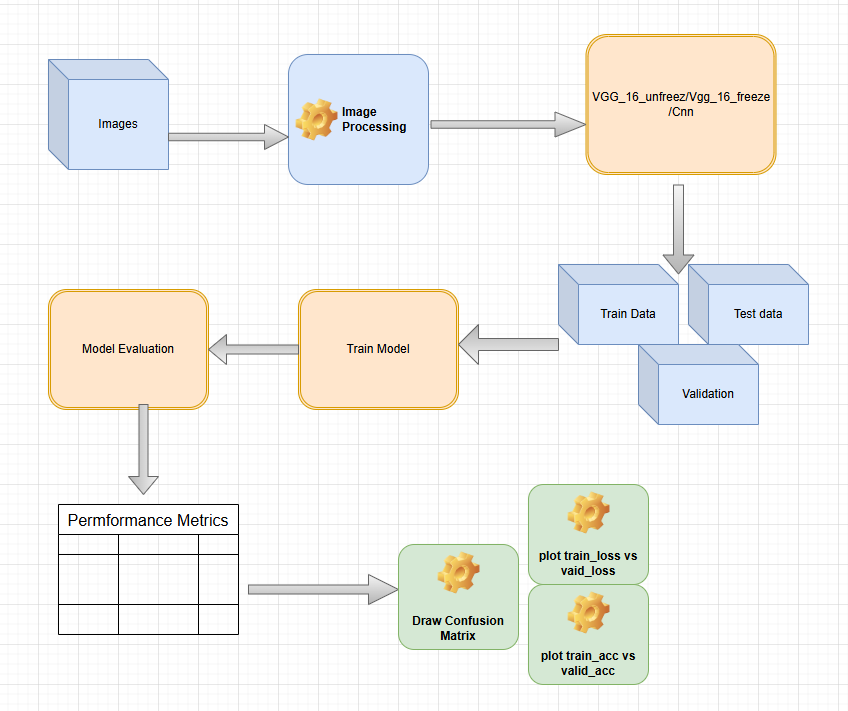
\includegraphics[width=1\linewidth]{common_workflow.png}
  \caption{Workflow Step}
  \label{fig:workflow1}
\end{figure}

\subsection{Step 1: Data Collection}

The first step involves collecting the dataset, which consists of images categorized into four classes: Closed, Open, No Yawn, and Yawn. This dataset is crucial for training and evaluating the models.

\subsection{Step 2: Data Preprocessing}

In this step, the collected images are preprocessed to ensure consistency and improve model performance. Preprocessing includes resizing, cropping, and normalization using \texttt{torchvision.transforms}. Data augmentation techniques are also applied to enhance the dataset's diversity.

\subsection{Step 3: Model Training}

The preprocessed data is then used to train the models. Various model architectures, such as VGG-16 with Batch Normalization, VGG-16 with Unfreezing and Learning Rate Scheduler, and a Lightweight CNN, are employed. Each model is fine-tuned and optimized for the task.

\subsection{Step 4: Model Evaluation}

After training, the models are evaluated using validation data. The performance metrics, such as accuracy and loss, are tracked and analyzed to determine the effectiveness of each model.


\section{Model Architectures}

\subsection{Model 1: VGG-16 with Batch Normalization}

The first model is based on the VGG-16 architecture with batch normalization. The model is pre-trained on ImageNet and fine-tuned for the DDD task. The last three convolutional layers are unfrozen to allow fine-tuning.

\begin{verbatim}
vgg16 = models.vgg16_bn(weights=models.VGG16_BN_Weights.DEFAULT)  # Use pretrained weights

# Freeze training for all layers in the feature extractor
for param in vgg16.features.parameters():
    param.requires_grad = False

# Unfreeze the last three convolutional layers
conv_layers_to_unfreeze = []
for i in range(len(vgg16.features) - 1, -1, -1):  # Traverse in reverse
    if isinstance(vgg16.features[i], nn.Conv2d):
        conv_layers_to_unfreeze.append(i)
    if len(conv_layers_to_unfreeze) == 3:
        break

# Unfreeze these layers
for i in conv_layers_to_unfreeze:
    for param in vgg16.features[i].parameters():
        param.requires_grad = True

# Modify the classifier to adapt to the number of classes
num_features = vgg16.classifier[6].in_features  # Get input features of the last layer
features = list(vgg16.classifier.children())[:-1]  # Remove last layer
features.append(nn.Linear(num_features, 4))  # Add a new layer for 4 classes
vgg16.classifier = nn.Sequential(*features)  # Replace the classifier
vgg16 = vgg16.to(device)
\end{verbatim}

\subsection{Model 2: VGG-16 with Unfreezing and Learning Rate Scheduler}

The second model is similar to the first but includes a learning rate scheduler to adjust the learning rate based on the validation loss.

\begin{verbatim}
criterion = nn.CrossEntropyLoss()
optimizer = optim.Adam(vgg16.parameters(), lr=0.0001, weight_decay=0.01)
exp_lr_scheduler = lr_scheduler.ReduceLROnPlateau(optimizer, mode='min', factor=0.5, patience=3)
\end{verbatim}

\subsection{Model 3: Lightweight CNN}

The third model is a lightweight CNN designed from scratch to balance computational efficiency and accuracy.

\begin{verbatim}
class LightWeightCNN(nn.Module):
    def __init__(self):
        super(LightWeightCNN, self).__init__()
        self.conv1 = nn.Conv2d(in_channels=3, out_channels=32, kernel_size=3, stride=1, padding=1)
        self.conv2 = nn.Conv2d(in_channels=32, out_channels=64, kernel_size=3, stride=1, padding=1)
        self.conv3 = nn.Conv2d(in_channels=64, out_channels=128, kernel_size=3, stride=1, padding=1)
        self.conv4 = nn.Conv2d(in_channels=128, out_channels=128, kernel_size=3, stride=1, padding=1)
        self.conv5 = nn.Conv2d(in_channels=128, out_channels=128, kernel_size=3, stride=1, padding=1)
        self.pool = nn.MaxPool2d(kernel_size=2, stride=2)
        self.fc1 = nn.Linear(in_features=128*7*7, out_features=1024)
        self.fc2 = nn.Linear(in_features=1024, out_features=4)
        self.dropout = nn.Dropout2d(0.2)
        self.dropout1 = nn.Dropout(0.2)

    def forward(self, x):
        x = self.dropout(self.pool(F.relu(self.conv1(x))))
        x = self.dropout(self.pool(F.relu(self.conv2(x))))
        x = self.dropout(self.pool(F.relu(self.conv3(x))))
        x = self.pool(F.relu(self.conv4(x)))
        x = self.pool(F.relu(self.conv5(x)))
        x = x.view(-1, 128*7*7)
        x = self.dropout1(x)
        x = F.relu(self.fc1(x))
        x = self.dropout1(x)
        x = self.fc2(x)
        return x
\end{verbatim}

\section{Training}

The models are trained using the following parameters:

\begin{itemize}
    \item \textbf{Optimizer:} SGD with learning rate 0.01 for the lightweight CNN, and Adam with learning rate 0.0001 for the VGG-16 models.
    \item \textbf{Loss Function:} CrossEntropyLoss
    \item \textbf{Epochs:} 50
\end{itemize}

Training and validation losses and accuracies are tracked and printed for each epoch. The models are saved if the validation loss decreases.
\chapter{Results}  % Now \chapter will work

\section{Evaluation Metrics}

The models' performance is evaluated using the following metrics:

\begin{itemize}
    \item \textbf{Accuracy:} Measures the proportion of correctly classified instances out of the total instances.
    \item \textbf{Precision:} Measures the proportion of true positive instances out of the total predicted positive instances.
    \item \textbf{Recall:} Measures the proportion of true positive instances out of the total actual positive instances.
    \item \textbf{F1 Score:} The harmonic mean of precision and recall, providing a single metric that balances both.
\end{itemize}

The table below summarizes the evaluation metrics for the models:

\begin{table}[htbp]
  \centering
  \caption{Evaluation Metrics for the Models}
  \vspace{0.5cm}  % Adjust the space here if needed
  \begin{tabular}{@{\hskip 5pt} l @{\hskip 10pt} c @{\hskip 10pt} c @{\hskip 10pt} c @{\hskip 10pt} c @{\hskip 5pt}}
  \toprule
  \textbf{Model} & \textbf{Accuracy} & \textbf{Precision} & \textbf{Recall} & \textbf{F1 Score} \\
  \midrule
  VGG-16 Fine-tuned  & 0.997691 & 0.997712 & 0.997691 & 0.997691 \\
  VGG-16  & 0.993072 & 0.993093 & 0.993072 & 0.993072 \\
  CNN        & 0.969977 & 0.969997 & 0.969977 & 0.969977 \\
  \bottomrule
  \end{tabular}
\end{table}
\newpage % Forces the next section to start on a new page

\section{VGG-16 Fine-tuned}

\subsection{Training and Validation Loss}

\begin{figure}[htbp]
\centering
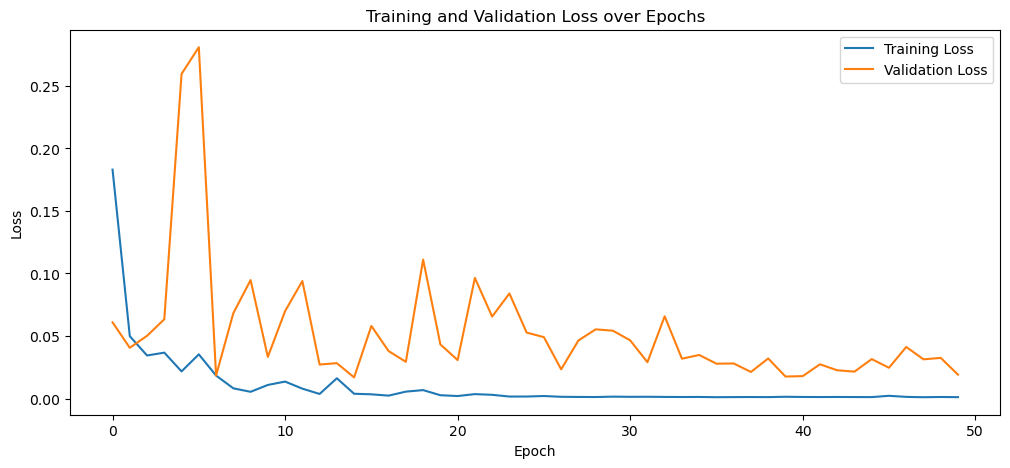
\includegraphics[width=0.8\textwidth]{train_val_loss_vgg16_uf.png}
\caption{Training and Validation Loss for VGG16 Fine-tuned (last 3 layers)}
\end{figure}

\subsection{Training and Validation Accuracy}

\begin{figure}[htbp]
\centering
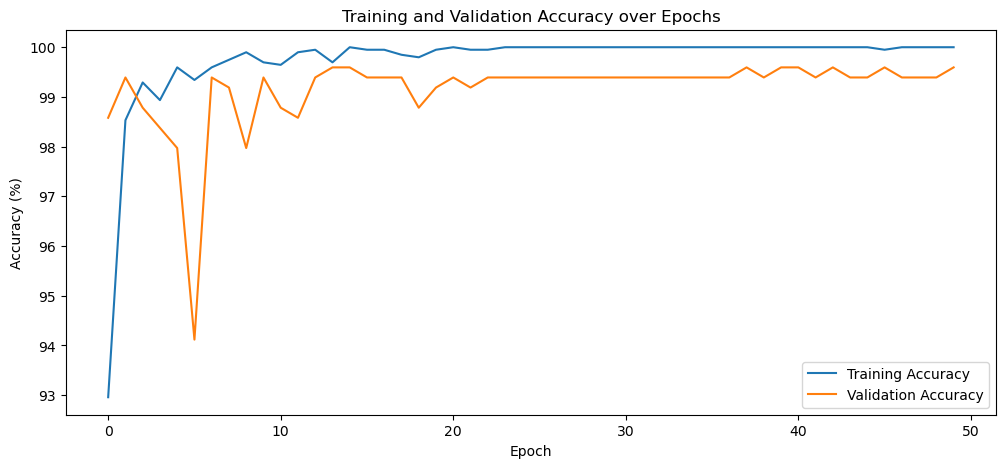
\includegraphics[width=0.8\textwidth]{train_val_acc_vgg16_uf.png}
\caption{Training and Validation Accuracy for VGG16 Fine-tuned (last 3 layers)}
\end{figure}

\newpage % Forces the next section to start on a new page

\section{VGG-16 with All Convolutional Layers Frozen}

\subsection{Training and Validation Loss}

\begin{figure}[htbp]
\centering
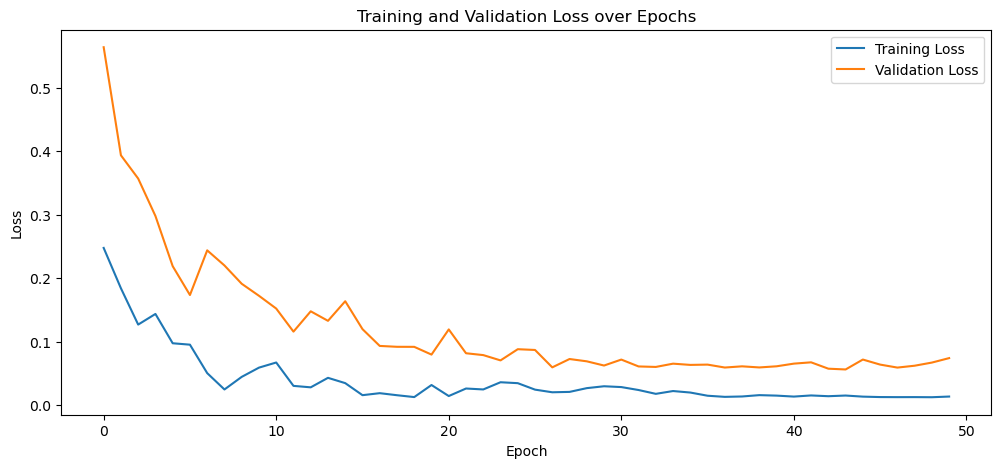
\includegraphics[width=0.8\textwidth]{train_val_err_vgg16.png}
\caption{Training and Validation Loss for VGG16 with Learning Rate Scheduler}
\end{figure}

\subsection{Training and Validation Accuracy}

\begin{figure}[htbp]
\centering
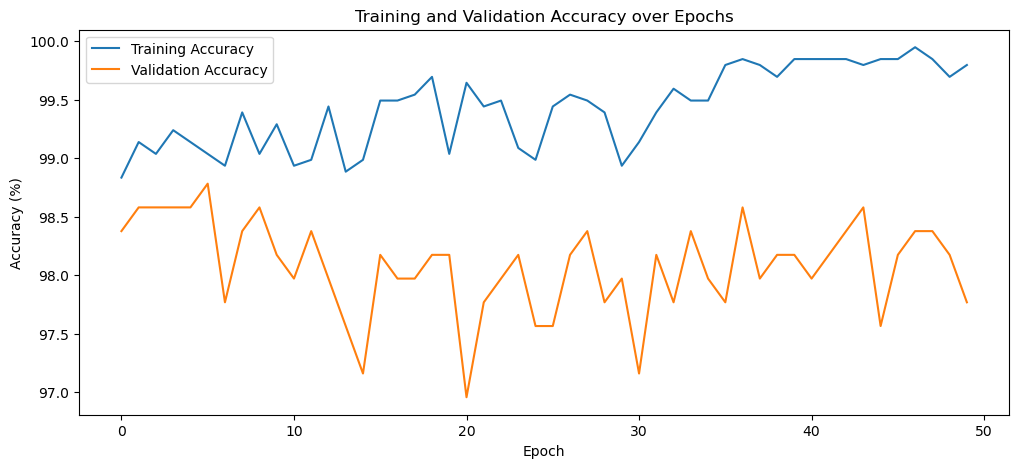
\includegraphics[width=0.8\textwidth]{train_val_acc_vgg16.png}
\caption{Training and Validation Accuracy for VGG16 with Learning Rate Scheduler}
\end{figure}

\newpage % Forces the next section to start on a new page

\section{Lightweight CNN}

\subsection{Training and Validation Loss}

\begin{figure}[htbp]
\centering
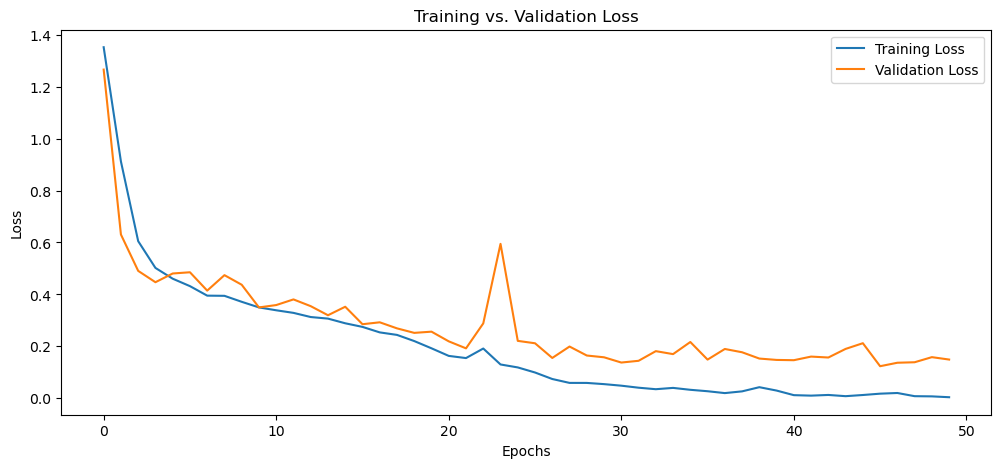
\includegraphics[width=0.8\textwidth]{train_valid_err_cnn.png}
\caption{Training and Validation Loss for Lightweight CNN}
\end{figure}

\subsection{Training and Validation Accuracy}

\begin{figure}[htbp]
\centering
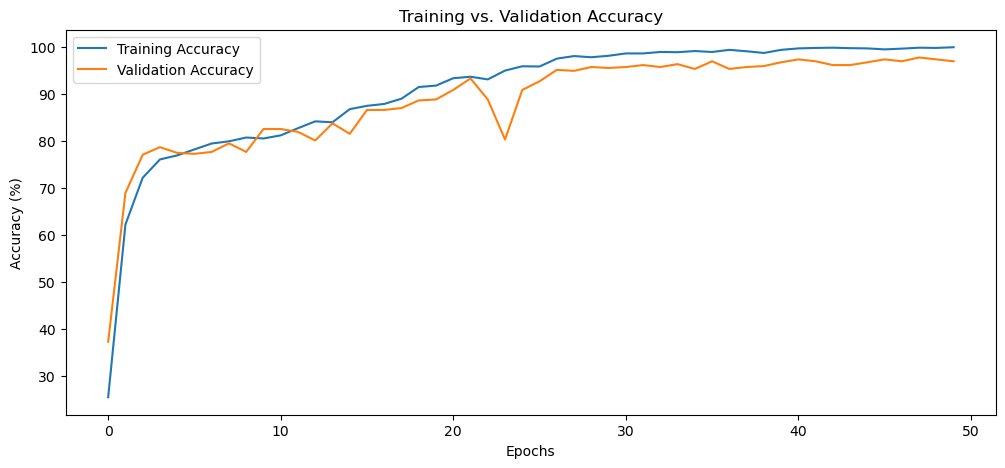
\includegraphics[width=0.8\textwidth]{train_valid_acc_cnn.png}
\caption{Training and Validation Accuracy for Lightweight CNN}
\end{figure}

\newpage % Forces the next section to start on a new page

\section{Confusion Matrix}

\begin{figure}[htbp]
\centering
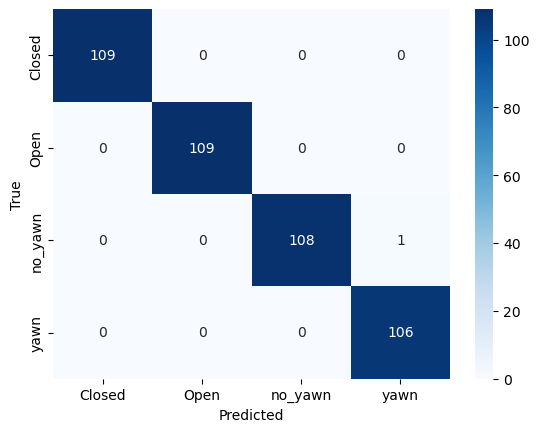
\includegraphics[width=0.8\textwidth]{vgg_16_unfreeze.png}
\caption{Confusion Matrix for VGG16 with Last 3 Convolutional Layers Unfrozen}
\end{figure}

\begin{figure}[htbp]
\centering
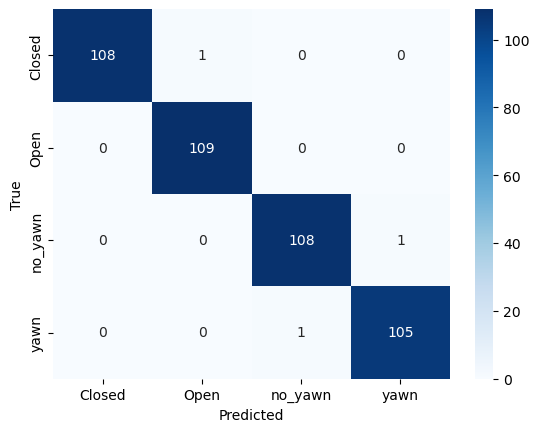
\includegraphics[width=0.8\textwidth]{vgg_16_freeze.png}
\caption{Confusion Matrix for VGG16 with All Convolutional Layers Frozen}
\end{figure}

\begin{figure}[htbp]
\centering
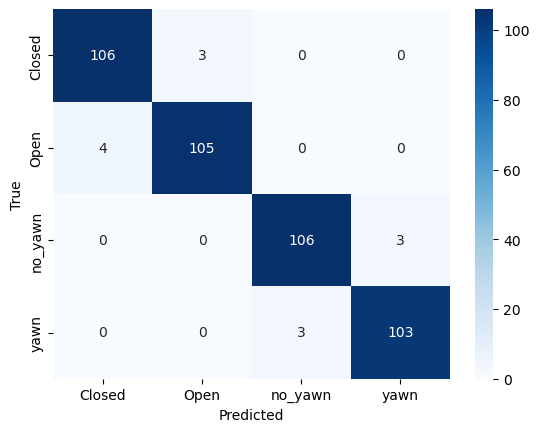
\includegraphics[width=0.8\textwidth]{conf_cnn.png}
\caption{Confusion Matrix for Lightweight CNN}
\end{figure}

\chapter{Conclusion and Future Work}

\section{Conclusion}

In this study, we developed and evaluated several models for detecting driver drowsiness and distraction. The models included VGG16 with Batch Normalization, VGG16 with Learning Rate Scheduler, and a Lightweight CNN. The performance of these models was assessed using various evaluation metrics, including accuracy, precision, recall, and F1 score.

The results demonstrated that the VGG16 with Batch Normalization model achieved the highest accuracy, precision, recall, and F1 score among the models evaluated. The Lightweight CNN model, while slightly less accurate, offered a good balance between computational efficiency and performance, making it suitable for real-time applications in driver monitoring systems.

Overall, the models showed satisfactory performance in detecting driver drowsiness and distraction, indicating their potential for use in real-world applications. However, there were some limitations due to the combined dataset for eye and yawning detection, which led to a loss of information.

\section{Future Work}

To address the limitations and further improve the performance of the models, the following future work is proposed:

\begin{itemize}
    \item \textbf{Head Pose Estimation Model:} Develop and integrate a head pose estimation model that will run concurrently with the VGG16 model. By combining the results from both models, we can provide a more accurate assessment of the driver's risk level.
    \item \textbf{Separate Models for Eye and Yawning Detection:} Currently, the combined dataset for eye and yawning detection leads to a loss of information. For example, when a driver yawns, their eyes automatically close, which can confuse the model. To mitigate this, we propose creating separate models for eye detection and yawning detection. This approach will help preserve the distinct information for each task.
    \item \textbf{Data Collection:} To support the development of separate models for eye and yawning detection, we have already collected a large amount of data. Future work will involve further expanding this dataset to ensure robust training and evaluation of the models.
    \item \textbf{Data Augmentation:} Implement additional data augmentation techniques to increase the diversity of the training dataset and improve the robustness of the models.
    \item \textbf{Hyperparameter Tuning:} Perform extensive hyperparameter tuning to optimize the performance of the models.
    \item \textbf{Complex Architectures:} Explore more complex architectures or pre-trained models to enhance the accuracy and generalization capabilities of the models.
    \item \textbf{Real-time Implementation:} Develop and test real-time implementations of the models in actual driving scenarios to evaluate their performance in real-world conditions.
    \item \textbf{Multi-modal Data:} Incorporate multi-modal data, such as physiological signals (e.g., heart rate, eye movement) and environmental factors (e.g., road conditions, weather), to improve the accuracy and reliability of the models.
    \item \textbf{User Feedback:} Collect and analyze user feedback to identify areas for improvement and ensure the models meet the needs and expectations of end-users.
\end{itemize}

By addressing these areas, future research can further enhance the performance and applicability of driver drowsiness and distraction detection systems, contributing to improved road safety and reduced accident rates.



% \nocite{golub} \nocite{gerla}\nocite{m1}\nocite{chang}
\bibliographystyle{plain}
\bibliography{ref}

\end{document}
